\documentclass{standalone}
\usepackage{tikz}
\usetikzlibrary{shapes.geometric, arrows}
\usepackage{amsmath}

\tikzstyle{startstop} = [rectangle, rounded corners, 
minimum width=3cm, 
minimum height=1cm,
text centered, 
draw=black, 
fill=red!10]

\tikzstyle{io} = [trapezium, 
trapezium stretches=true,
trapezium left angle=70, 
trapezium right angle=110, 
minimum width=3cm, 
minimum height=1cm, text centered, 
draw=black, fill=blue!10]

\tikzstyle{process} = [rectangle, 
minimum width=5cm, 
minimum height=1cm, 
text centered, 
text width=5cm, 
draw=black, 
fill=orange!10]

\tikzstyle{decision} = [diamond, 
minimum width=3cm, 
minimum height=1cm, 
text centered, 
draw=black, 
fill=green!10]
\tikzstyle{arrow} = [thick,->,>=stealth]
\begin{document}

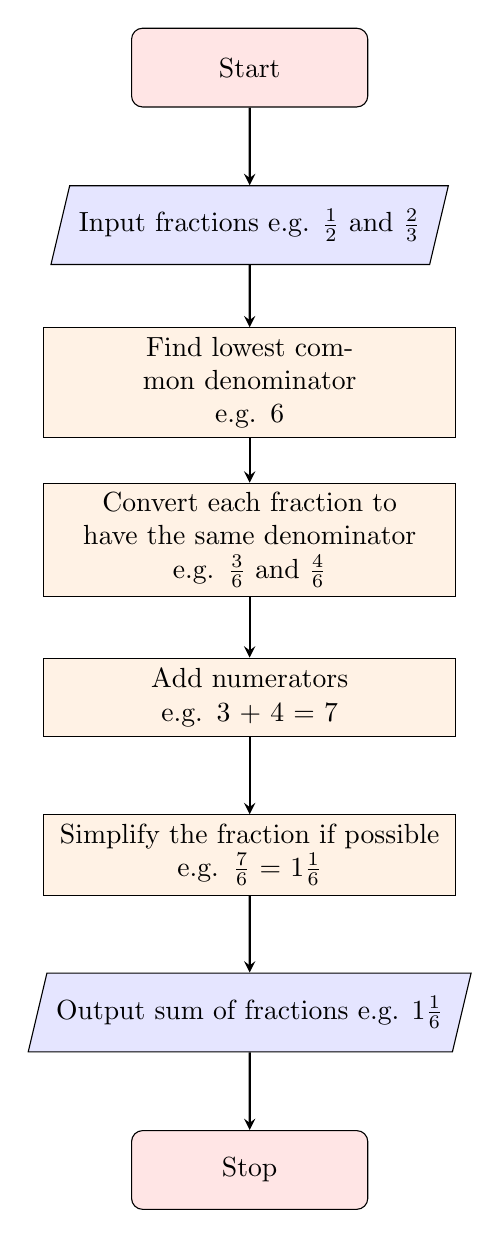
\begin{tikzpicture}[node distance=2cm]

\node (start) [startstop] {Start};
\node (in1) [io, below of=start] {Input fractions ~\\ e.g. $\frac{1}{2}$ and $\frac{2}{3}$};
\node (pro1) [process, below of=in1] {Find lowest common denominator \\ e.g. 6};
\node (pro2) [process, below of=pro1] {Convert each fraction to have the same denominator \\ e.g. $\frac{3}{6}$ and $\frac{4}{6}$};
\node (pro3) [process, below of=pro2] {Add numerators \\ e.g. 3 + 4 = 7};
\node (pro4) [process, below of=pro3] {Simplify the fraction if possible \\ e.g. $\frac{7}{6}$ = 1$\frac{1}{6}$};
\node (out1) [io, below of=pro4] {Output sum of fractions ~\\ e.g. 1$\frac{1}{6}$};
\node (stop) [startstop, below of=out1] {Stop};

\draw [arrow] (start) -- (in1);
\draw [arrow] (in1) -- (pro1);
\draw [arrow] (pro1) -- (pro2);
\draw [arrow] (pro2) -- (pro3);
\draw [arrow] (pro3) -- (pro4);
\draw [arrow] (pro4) -- (out1);
\draw [arrow] (out1) -- (stop);

\end{tikzpicture}
\end{document}
